% License: CC BY-SA
% Authors: See the authors below and see also acknowledgement for authors of some images or research

\documentclass[25pt, margin=0mm, innermargin=25mm, blockverticalspace=25mm, colspace=25mm, subcolspace=8mm]{tikzposter}
\geometry{paperwidth=63in,paperheight=42in}

% to stretch boxes over whole paper with custor paper size
\makeatletter
\setlength{\TP@visibletextwidth}{\textwidth-2\TP@innermargin}
\setlength{\TP@visibletextheight}{\textheight-2\TP@innermargin}
\makeatother

% Fira Sans, GRASS GIS branding sans serif font
\usepackage{FiraSans}
\renewcommand*\oldstylenums[1]{{\firaoldstyle #1}}

% EB Garamond, GRASS GIS branding serif font
% note that EB Garamond does not have bold
\usepackage[cmintegrals,cmbraces]{newtxmath}
\usepackage{ebgaramond-maths}

% might be needed for both font packages
\usepackage[T1]{fontenc}

% uncomment for all sans serif
% \renewcommand{\familydefault}{\sfdefault}

\usepackage{setspace}

\usepackage[utf8]{inputenc}
\usepackage{wrapfig}
\usepackage[hidelinks]{hyperref}

% For bibliography styling
%% TODO: all names should be abbreviated
\usepackage{natbib}

\definecolor{textcolor}{HTML}{000000}

\definecolor{titleTextColor}{HTML}{000000}
\definecolorpalette{grassColorPalette} {
  \definecolor{colorOne}{HTML}{419041}
  % \definecolor{colorTwo}{HTML}{cccccc}
  \definecolor{colorTwo}{HTML}{dddddd}
  \definecolor{colorThree}{HTML}{F1B52D}
  % \definecolor{colorThree}{HTML}{EFA126}
}

\usetheme{Default}
\usetitlestyle{Empty}
\usecolorstyle[colorPalette=grassColorPalette]{Britain}
\colorlet{backgroundcolor}{white}

\title{
\Huge
\textcolor{titleTextColor}{
\textsf{
% \textbf{
\fontsize{130}{100}\selectfont
\textbf{GRASS}\,{\firalight GIS}: A General-purpose Geospatial Research Tool
% }
}
}
}

\newlength{\grasslogoheight}
\setlength{\grasslogoheight}{0.09\textheight}
\newlength{\instlogoheight}
\setlength{\instlogoheight}{0.33\grasslogoheight}

% \setlength{\blocktitleheight}{0.02\textheight}

% style for institute numbers
\newcommand{\inst}[1]{\hspace{2pt}$^{\mbox{\normalsize#1}}$\hspace{-7pt}}
\newcommand{\instlist}[1]{\hspace{1pt}$^{\mbox{\normalsize#1}}$\hspace{2pt}}

\author{
Helena Mitasova\inst{1},
Vaclav Petras\inst{1}\,*\hspace{-7pt},
Anna Petrasova\inst{1},
\&
Markus Neteler\inst{2}
\\
% AGU allows to specify a scientific team, but it does not seem to fit
% with our case 100%; simply using formatting which is in the AGU program
% (but adding note)
Scientific Team: GRASS GIS Development Team**
}
\institute{
\large
\instlist{1}Center for Geospatial Analytics, North Carolina State University, USA;
\instlist{2}mundialis GmbH \& Co. KG, Germany;
*Corresponding author: wenzeslaus@gmail.com, vpetras@ncsu.edu;
% using Black Duck Open Hub to ``guestimate'' that
**Includes over 10 other members of the core team and numerous other contributors
\\[1.7cm]

\includegraphics[height=3cm]{ncstate}%
\hspace{1cm}%

\includegraphics[height=3cm]{cga}%
\hspace{3cm}%

\includegraphics[height=3.4cm]{mundialis}%
}

\hypersetup
{
    pdfauthor={H. Mitasova, V. Petras, A. Petrasova, M. Neteler},
    pdfsubject={AGU Fall Meeting 2018 Poster},
    pdftitle={GRASS GIS: A General-purpose Geospatial Research Tool},
    pdfkeywords={GIS, algorithms, methods, preservation, science, reproducibility}
}

% \usetemplate{1}
% \setinstituteshift{1}

% \setblocktitleheight{2}
% \setblockspacing{1}

\graphicspath{{images/}{logos/}}

\newcommand{\blocktitlewrap}[1]{\textnormal{\textsf{\textsc{\huge#1}}}}
% it is not possible (?) to change block title in the class, using wrapper
% the command introduced using:
%   sed -i 's/\\block{\([^}]*\)}/\\block{\\blocktitlewrap{\1}}/g' main.tex

\newcommand{\CustomBlockFontSize}{\LARGE}

% bullet point style
\renewcommand{\labelitemi}{\textcolor{gray}{$\bullet$}\hspace{0.5ex}}

% GRASS module
\newcommand{\gmodule}[1]{\href{http://grass.osgeo.org/grass74/manuals/#1.html}{\emph{#1}}}
\newcommand{\gamodule}[1]{\href{http://grass.osgeo.org/grass74/manuals/addons/#1.html}{\emph{#1}}}
\newcommand{\gmodulenolink}[1]{\emph{#1}}

\begin{document}

\node[above left,opacity=0.99,inner sep=0pt,outer sep=6cm] at (bottomleft -| topright)%
  {
\includegraphics[width=0.2\paperwidth]{grass}};

\maketitle[width=0.92\textwidth]

% \maketitle
% \addlogo[north west]{(2,-1)}{9cm}{images/Grass_GIS}
%Please insert your institution logo here
% \addlogo[north east]{(-2,-2.5)}{4cm}{images/logo_FEM_CRI}
% \addlogo[north east]{(-2,-5.5)}{4cm}{images/NC_State_Seal}
% \addlogo[north east]{(-8,-2.5)}{4cm}{images/Logo_cvut}
% \addlogo[north east]{(-8,-6.5)}{4cm}{images/IWMI_logo}
% \addlogo[north east]{(-2,-10.5)}{4cm}{images/logo_ec-jrc}

\begin{columns}

% Abstract
%
% GRASS GIS (grass.osgeo.org) is an open source software for geospatial analysis,
% remote sensing, general geoprocessing and visualization. It is a
% community-driven project with over 35 years of continuous software development
% based on scientific expertise from many geospatial fields. It is characterized
% by long-term releases, stable APIs, and emphasis on science. GRASS GIS
% distribution strives to provide single integrated environment for 2D and 3D
% raster analysis, image processing, vector data analysis, and spatio-temporal
% data processing. It supports large raster files (billions of cells), vector
% topology, coupling with databases, and 64 bit memory. New code based on recent
% research is typically contributed to GRASS GIS Addons repository. Mature, widely
% used code is then moved to the main code base to maximize integration and
% availability. Whether it is addons or the main code base, code is usually
% maintained by the community and preserved in long term even in cases when the
% original author no longer supports the code. To support the needs of scientists,
% the documentation includes not only links to the source code, its history, and
% its authors, but also links to research papers that describe the algorithms
% implemented in the modules.
%
% Code is not only maintained but also extended and improved. For example,
% watershed and stream extraction using least cost path approach was implemented
% in 1989 and extended for massive datasets in 2011. Similarly, vector topology
% cleaning was introduced in 2002, updated over time and substantially improved in
% 2016. Another example is a solar energy module available since 1993 and
% parallelized in 2017. The current stable version of GRASS GIS 7.4 provides new
% features for geosciences such as temporal framework with temporal algebra for
% large time-series processing, fusion of elevation models from various sensors,
% 3D flows, landform detection, image segmentation, simplified batch processing,
% and integrated Python editor among others. GRASS GIS runs in various
% environments including Linux, Mac, Windows, Docker, Raspberry Pi, and on HPC
% clusters. The modules are written in Python, C, or C++. Besides command line
% interface, GRASS GIS provides a graphical user interface, a Python API, and a C
% API. Interfaces with other languages such as R and Ruby are supplied by
% collaborating communities.

%%%%%%%%%%%%%%%%%%%%%%%%%%%%%%%%%%%%%%%%%%%%%%%%%%%%%%%%%%%%%%%%%%%%%
%%%%%%%%%%%%%%%%%%%%%%%%%%%%%%%%%%%%%%%%%%%%%%%%%%%%%%%%%%%%%%%%%%%%%
%%%%%%%%%%%%%%%%%%%%%%%%%%%%%%%%%%%%%%%%%%%%%%%%%%%%%%%%%%%%%%%%%%%%%
%%%%%%%%%%%%%%%%%%%%%%%%%%%%%%%%%%%%%%%%%%%%%%%%%%%%%%%%%%%%%%%%%%%%%
\column{0.25}

%%%%%%%%%%%%%%%%%%%%%%%%%%%%%%%%%%%%%%%%%%%%%%%%%%%%%%%%%%%%%%%%%%%%%%%%%%%%%%%
\block{\blocktitlewrap{Why GRASS GIS as a Tool?}}{

\CustomBlockFontSize

Multiple researchers for over three decades
contributed code,
published associated papers,
implemented other's papers
and improved and built on each others work.

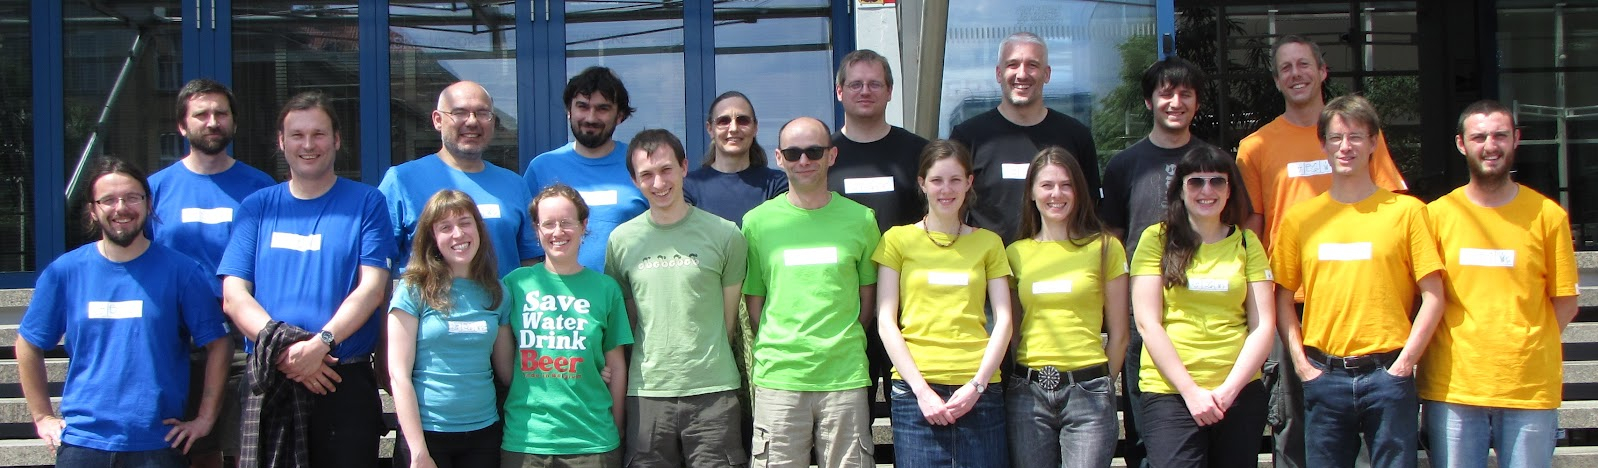
\includegraphics[width=\linewidth]{grass_team}

\begin{itemize}
% Basic Topics
 \item Community-driven project
 \item Long-term releases, stable APIs and emphasis on science
 \item Single integrated environment for 2D and 3D raster analysis, image processing, vector data analysis and spatio-temporal data processing
% GRASS GIS
% distribution strives to provide single integrated environment for 2D and 3D
% raster analysis, image processing, vector data analysis and spatio-temporal
% data processing. It supports large raster files (billions of cells), vector
% topology, coupling with databases and 64 bit memory.
%  \item To support the needs of scientists, the documentation includes not only links to the source code, its history and
% its authors, but also links to research papers that describe the algorithms
% implemented in the modules.
\end{itemize}


}

%%%%%%%%%%%%%%%%%%%%%%%%%%%%%%%%%%%%%%%%%%%%%%%%%%%%%%%%%%%%%%%%%%%%%%%%%%%%%%%
\block{\blocktitlewrap{Why GRASS GIS as a Platform?}}{

\CustomBlockFontSize

Contributed code is maintained and extended by community
and prevails even in cases when the original author cannot support its users.

\begin{itemize}
 \item New code typically contributed to Addons repository.
 \item Mature code is moved to the main code base.
 \item Both main code base and Addons maintained by the community.
\end{itemize}

}



%%%%%%%%%%%%%%%%%%%%%%%%%%%%%%%%%%%%%%%%%%%%%%%%%%%%%%%%%%%%%%%%%%%%%%%%%%%%%%%%
\block{\blocktitlewrap{Example: Vector Network Analysis}}{

\CustomBlockFontSize

\begin{itemize}
 \item Radim Blazek introduced several modules for vector network analysis in 2003
       including shortest path analysis (\gmodule{v.net.path}) and traveling salesman (\gmodule{v.net.salesman}).
 \item The number of available modules increased to almost 20.
 \item Stepan Turek implemented turns support into all relevant vector network modules in 2014.
%  \item Since version 7.0 fine control over node costs available.
% combination with r.cost/r.walk workflows \citep{Petrasova2014}
\end{itemize}

\bigskip

\centering
\begin{minipage}{0.9\linewidth}
\begin{center}
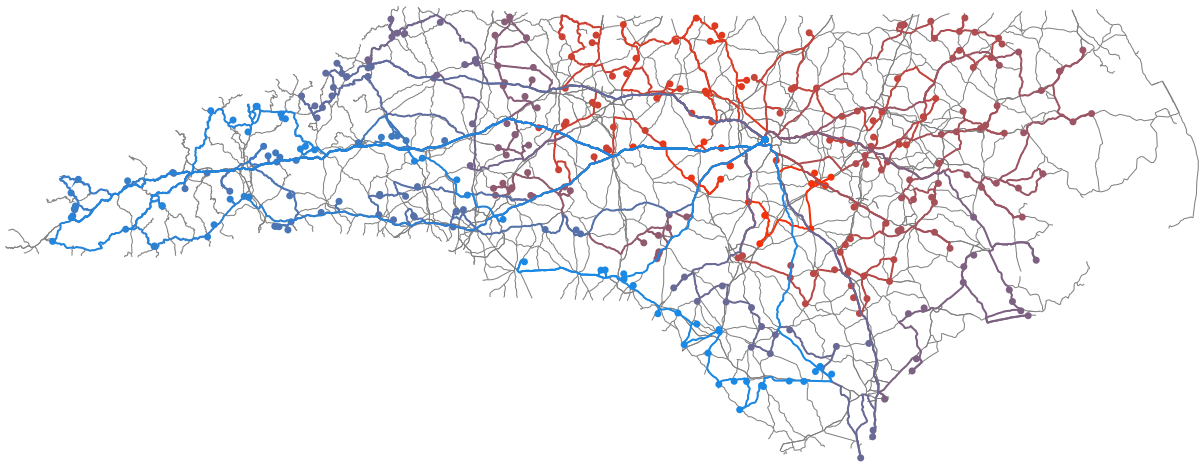
\includegraphics[width=\textwidth]{network_trips}
A series of trips to collect samples across North Carolina, USA
for water quality measurements
as part of the Polyfluorinated Alkyl Substance Testing (PFAST) project.
Trips are distinguished by color and were computed using multiple
iterations of traveling salesman (\gmodule{v.net.salesman}).
\end{center}
\end{minipage}

}


%%%%%%%%%%%%%%%%%%%%%%%%%%%%%%%%%%%%%%%%%%%%%%%%%%%%%%%%%%%%%%%%%%%%%
%%%%%%%%%%%%%%%%%%%%%%%%%%%%%%%%%%%%%%%%%%%%%%%%%%%%%%%%%%%%%%%%%%%%%
%%%%%%%%%%%%%%%%%%%%%%%%%%%%%%%%%%%%%%%%%%%%%%%%%%%%%%%%%%%%%%%%%%%%%
%%%%%%%%%%%%%%%%%%%%%%%%%%%%%%%%%%%%%%%%%%%%%%%%%%%%%%%%%%%%%%%%%%%%%
\column{0.25}

%%%%%%%%%%%%%%%%%%%%%%%%%%%%%%%%%%%%%%%%%%%%%%%%%%%%%%%%%%%%%%%%%%%%%
\block{\blocktitlewrap{Example: Spatio-Temporal Data Analysis}}{

\CustomBlockFontSize

\begin{itemize}
 \item The time dimension was introduced in version 7.0 \citep{Gebbert20141, gebbert2015grass}
 \item Time series accessed as space time datasets and as individual vectors or rasters.
 \item More than 50 modules available to manage, analyze, process and visualize space time datasets.
 \item More than 100,000 map layers can be now handled efficiently in GRASS GIS.
 \item Used for analysis of the European Climate Assessment \& Dataset ECA\&D \citep{Haylock2008_climate_series}
       and temperate climate zone identification \citep{Gebbert20141}.
 \item New temporal modules (e.g. \gmodule{t.rast.aggregate}) work beside well established \gmodule{r.series} module
       and specialized modules such as \gamodule{r.hants} implemented according to \cite{roerink2000reconstructing} or \gamodule{r.seasons}.
 \item Raster and vector temporal algebra can be used for tasks
       such as computing hydrothermal coefficient for a time series of climate data using the actual mathematical formula
       \citep{leppelt2015grass}.
\end{itemize}

\vspace*{1.5cm}

\begin{minipage}{\linewidth}
\centering
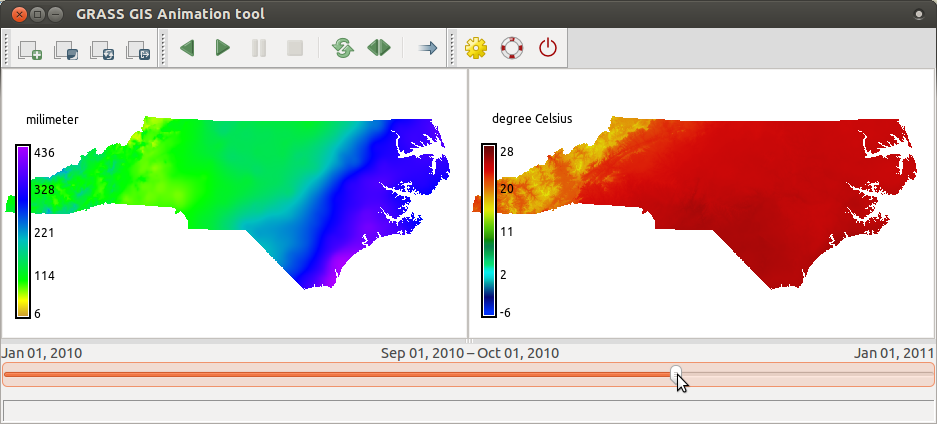
\includegraphics[width=.7\linewidth]{images/temporal_precip_temp}
\\
Creating a synchronized animation of monthly total precipitation and mean temperature for NC, USA
\end{minipage}

\vspace*{1cm}

}



%%%%%%%%%%%%%%%%%%%%%%%%%%%%%%%%%%%%%%%%%%%%%%%%%%%%%%%%%%%%%%%%%%%%%%%%%%%%%%%%
\block{\blocktitlewrap{References}}{

\vspace{-0.2cm}

\scriptsize
\setstretch{0.5}

% \newcommand{\blocksectiontitle}[1]{\subsubsection*{\textcolor{gray}{\textsf{#1}}}}
\newcommand{\blocksectiontitle}[1]{\textbf{#1}}

%\blocksectiontitle{References}
\begingroup
\renewcommand{\section}[2]{}%
\bibliographystyle{apalike}
\bibliography{poster}
\endgroup

}



%%%%%%%%%%%%%%%%%%%%%%%%%%%%%%%%%%%%%%%%%%%%%%%%%%%%%%%%%%%%%%%%%%%%%
%%%%%%%%%%%%%%%%%%%%%%%%%%%%%%%%%%%%%%%%%%%%%%%%%%%%%%%%%%%%%%%%%%%%%
%%%%%%%%%%%%%%%%%%%%%%%%%%%%%%%%%%%%%%%%%%%%%%%%%%%%%%%%%%%%%%%%%%%%%
%%%%%%%%%%%%%%%%%%%%%%%%%%%%%%%%%%%%%%%%%%%%%%%%%%%%%%%%%%%%%%%%%%%%%
\column{0.25}

%%%%%%%%%%%%%%%%%%%%%%%%%%%%%%%%%%%%%%%%%%%%%%%%%%%%%%%%%%%%%%%%%%%%%%%%%%%%%%%
\block{\blocktitlewrap{Example: Image Segmentations}}{

\CustomBlockFontSize

\begin{itemize}
% according to \cite{mumford1989optimal} and \cite{march1997variational}
 \item \gmodule{r.clump} for grouping pixels with the same integer values available since '80s.
       Now \gmodule{r.clump} handles multiple image bands and floating point values.
 \item \gamodule{r.smooth.seg} for noise reduction \citep{vitti2008free, vitti2012mumford}
 \item Region-growing image segmentation originally from Eric Momsen (2012)
       was improved by Markus Metz and included as \gmodule{i.segment} into version 7.0.
%        This replaced a multi-resolution classification module of the same name from 1992 \citep{zhuang1992image}.
 \item \gamodule{i.segment.hierarchical} by Pietro Zambelli based on \gmodule{i.segment} performs parallelized hierarchical segmentation.
 \item Rashad Kanavath and Markus Metz implemented SLIC Superpixels segmentation \citep{achanta2010epfl, achanta2012slic} in 2016 as \gmodule{i.superpixels.slic}.
\end{itemize}

\vspace*{0.7cm}

\begin{minipage}{0.5\linewidth}
\begin{center}
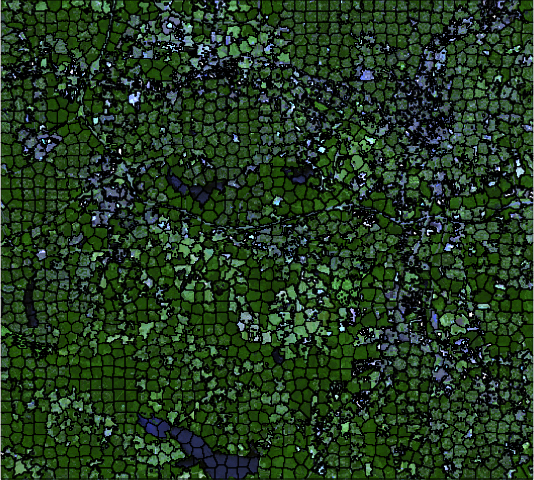
\includegraphics[width=\textwidth]{superpixels_slic_pseudo}
\end{center}
\end{minipage}
~
\begin{minipage}{0.5\linewidth}
\begin{center}
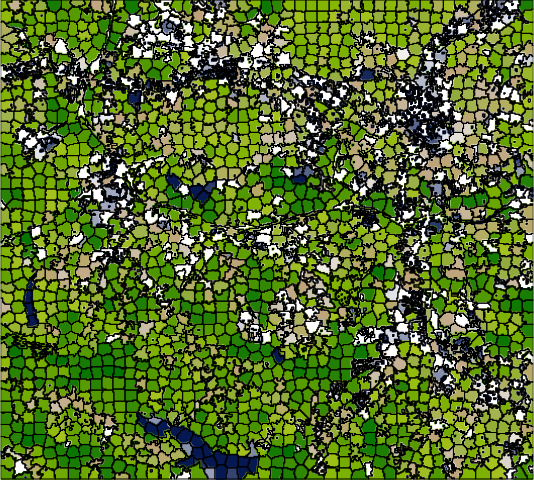
\includegraphics[width=\textwidth]{superpixels_slic_colored}
\end{center}
\end{minipage}
\vspace{2mm}
\begin{center}
Superpixels (black outlines) with pseudo-color and NDVI images, central Wake county, NC, USA
\end{center}

\vspace*{0cm}

}

%%%%%%%%%%%%%%%%%%%%%%%%%%%%%%%%%%%%%%%%%%%%%%%%%%%%%%%%%%%%%%%%%%%%%
%%%%%%%%%%%%%%%%%%%%%%%%%%%%%%%%%%%%%%%%%%%%%%%%%%%%%%%%%%%%%%%%%%%%%%%%%%%%%%%%%
\block{\blocktitlewrap{Example: Water, Floods and Erosion}}{

\CustomBlockFontSize

\begin{itemize}
 \item \gmodule{r.sim.water} module \citep{Mitas1998b}
       for simulating overland flow integrated into the Emergency Routing Decision Planning \citep{raghavan2014deploying}.
% TODO: paralelized
 \item \gmodule{r.watershed} for least cost path water accumulation from 1989
       and updated for massive data sets in 2011.
% TODO: refs
 \item \cite{Petrasova2014} utilized in \emph{Tangible Landscape}, a tangible GIS system,
       \gmodule{r.damflood}, a dam break inundation simulation by \cite{cannata2012two}.
\end{itemize}

% \bigskip

% \vspace*{0.5cm}

\centering

\begin{minipage}{0.485\linewidth}
\centering
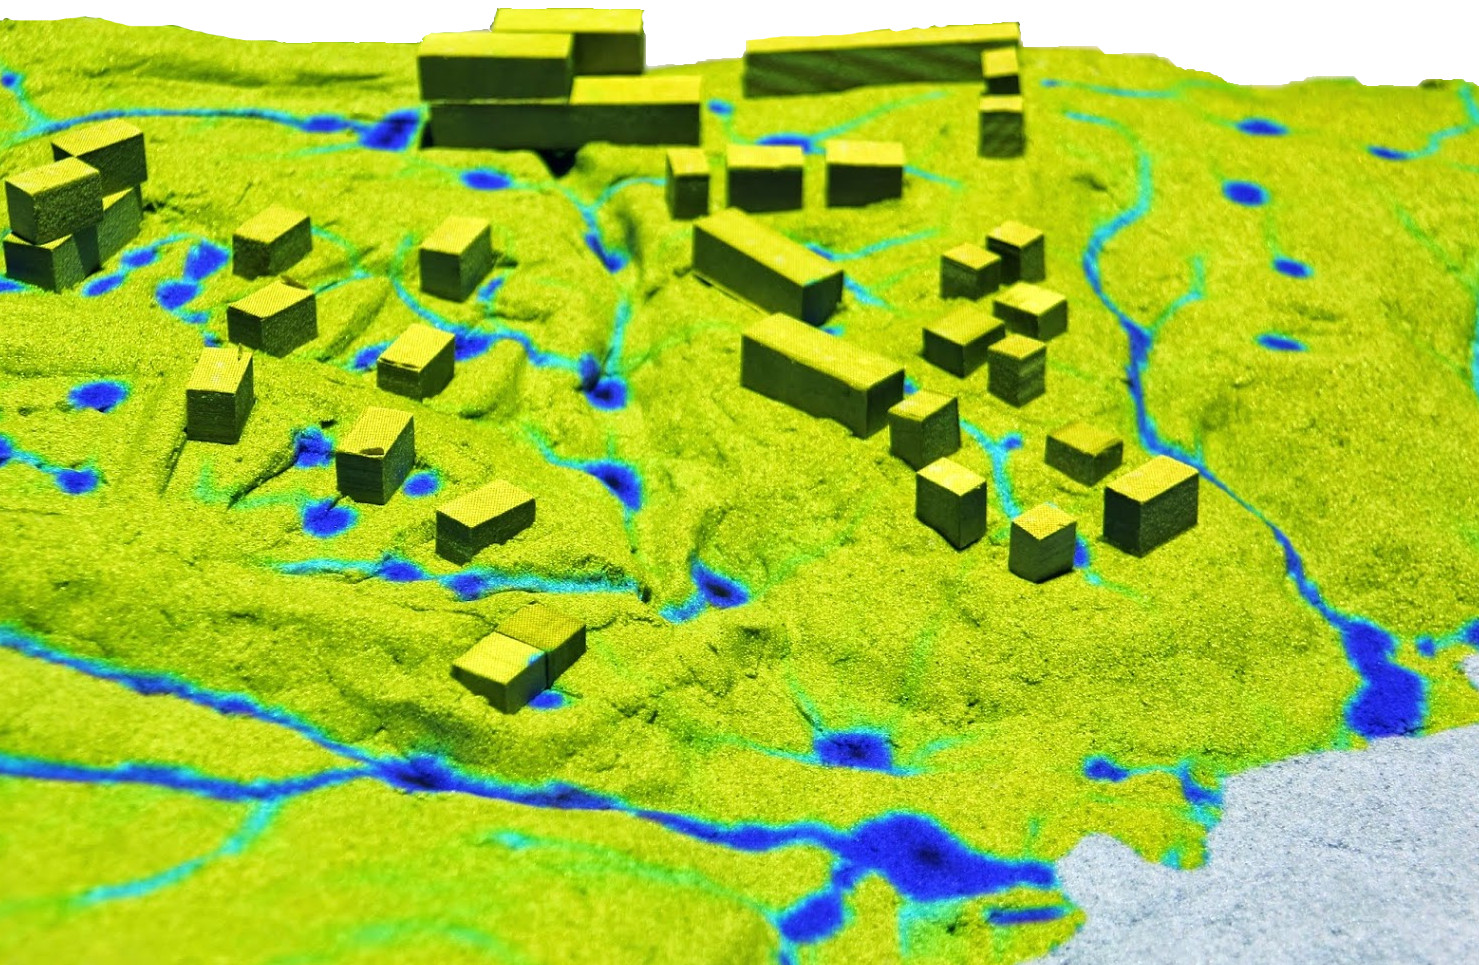
\includegraphics[width=0.7\textwidth]{rsimwater_architects}
\end{minipage}
~
\begin{minipage}{0.485\linewidth}
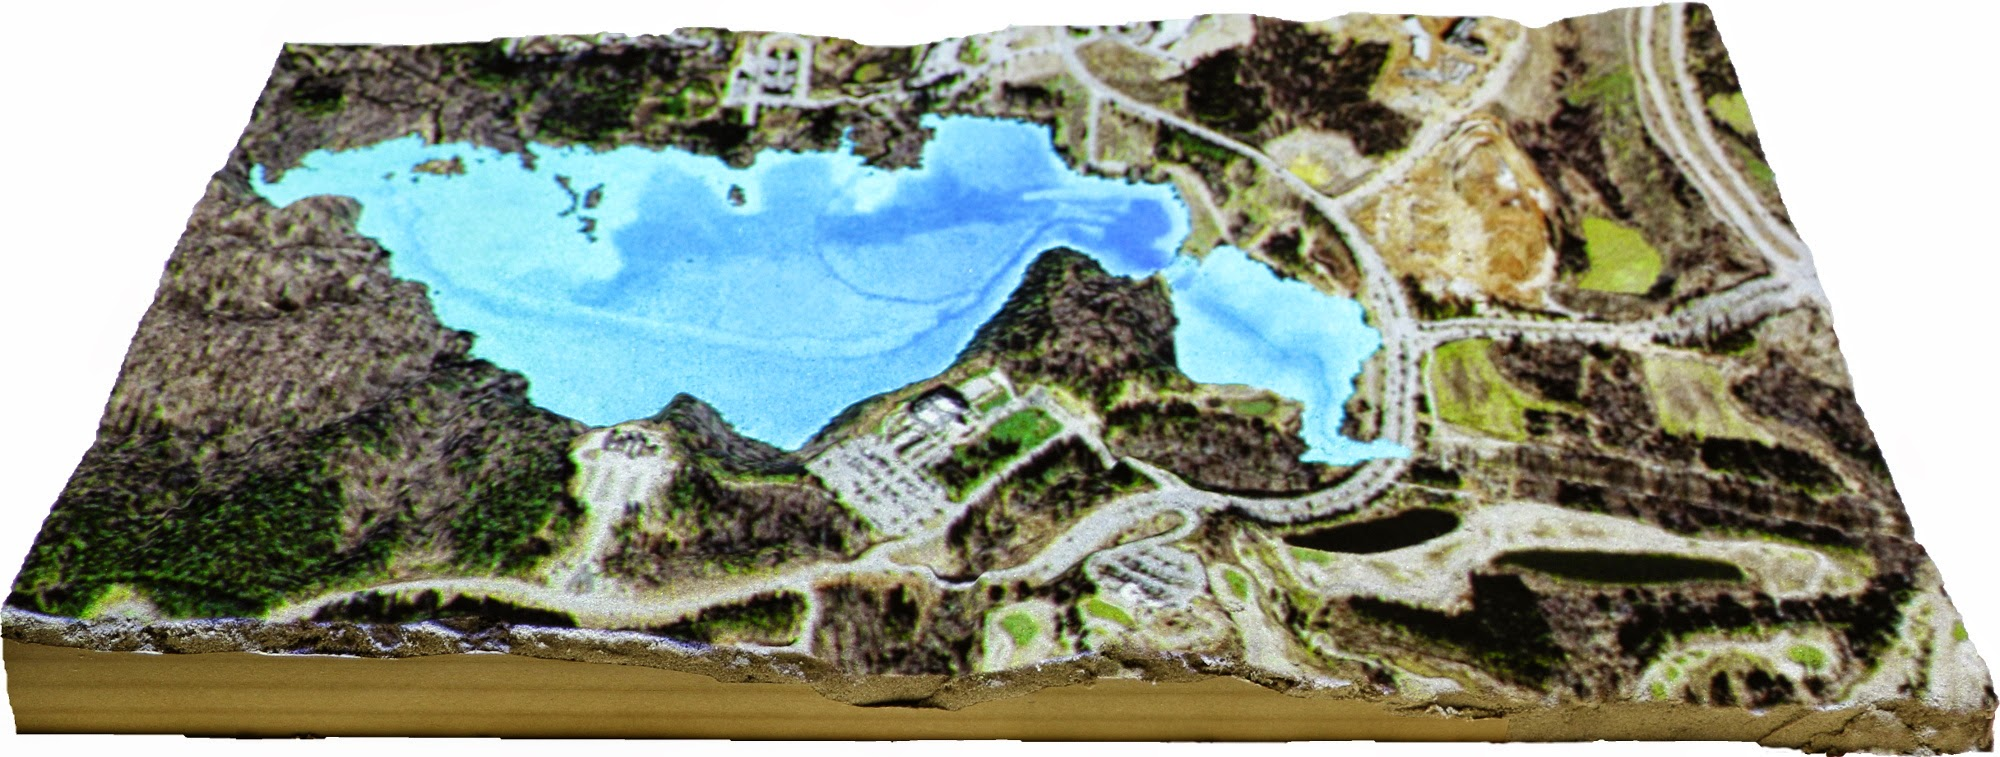
\includegraphics[width=\textwidth]{damflood_tangible}
\end{minipage}
\vspace{2mm}
\begin{center}
Overland flow simulated used for landscape
architecture design in Tangible Landscape environment (left)
and a dam breach on Lake Raleigh, NC, USA (right)
\end{center}


% \vspace*{1.4cm}
}

%%%%%%%%%%%%%%%%%%%%%%%%%%%%%%%%%%%%%%%%%%%%%%%%%%%%%%%%%%%%%%%%%%%%%
%%%%%%%%%%%%%%%%%%%%%%%%%%%%%%%%%%%%%%%%%%%%%%%%%%%%%%%%%%%%%%%%%%%%%
%%%%%%%%%%%%%%%%%%%%%%%%%%%%%%%%%%%%%%%%%%%%%%%%%%%%%%%%%%%%%%%%%%%%%
%%%%%%%%%%%%%%%%%%%%%%%%%%%%%%%%%%%%%%%%%%%%%%%%%%%%%%%%%%%%%%%%%%%%%
\column{0.25}

%%%%%%%%%%%%%%%%%%%%%%%%%%%%%%%%%%%%%%%%%%%%%%%%%%%%%%%%%%%%%%%%%%%%%
\block{\blocktitlewrap{Example: Lidar Data Processing}}{

\CustomBlockFontSize

\begin{itemize}
 \item Filtering of ground points was included
       in the \gmodule{v.lidar.edgedetection} group of modules.
% TODO: ref
% TODO: year
% v.lidar.correction Corrects the v.lidar.growing output. It is the last of the three algorithms for LIDAR .
% v.lidar.edgedetection Detects the object's edges from a LIDAR data set.
% v.lidar.growing Building contour determination and Region Growing algorithm for determining the building inside
 \item \gmodule{v.outlier} module serves as a base for a module \gamodule{v.lidar.mcc} implementing Multiscale Curvature Classification.
% TODO: ref
 \item \gmodule{v.surf.rst} (spatial interpolation) for developed in '90s;
       improved several times and parallelized for version 7.4.
% \citep{tracvsurfrst}
% TODO: different ref
% TODO: ref for paralelized
 \item Improved \gmodule{r.in.lidar} statistically analyzes large point clouds.
% TODO: base_raster, ref

\end{itemize}

\centering
\begin{minipage}{0.4\linewidth}
\centering
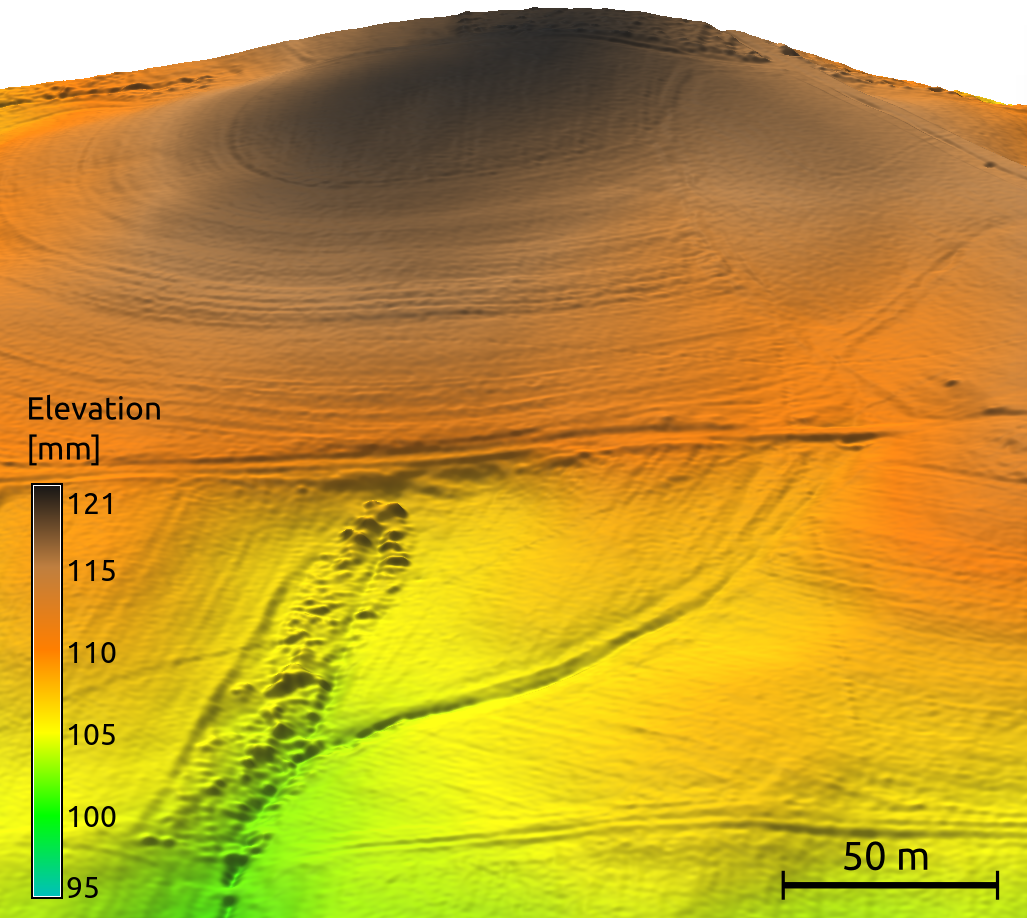
\includegraphics[width=0.7\textwidth]{elevation_lidar}
\end{minipage}
~
\begin{minipage}{0.55\linewidth}
\centering
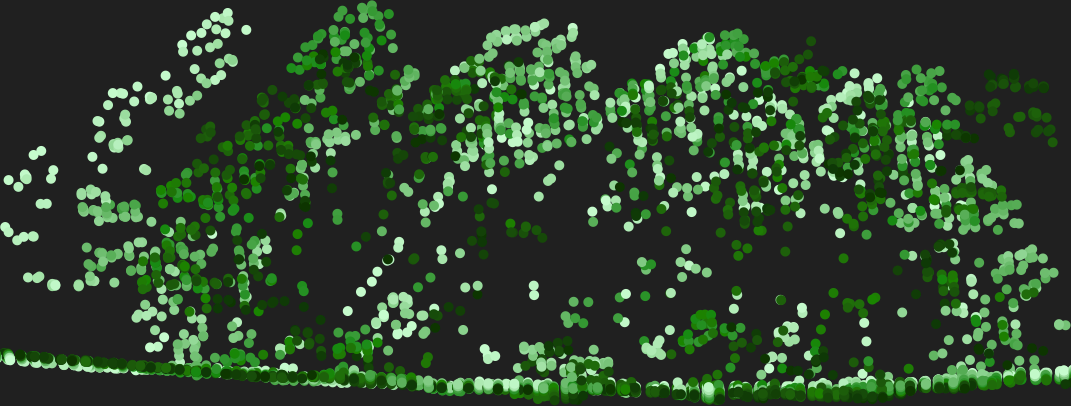
\includegraphics[width=\textwidth]{lidar_profile}
\end{minipage}
\vspace{2mm}
\begin{center}
Digital elevation model interpolated from lidar data shows tillage in an field in Raleigh, NC, USA
and a point cloud transect created with \gamodule{v.profile.points} shows tree structure
\end{center}

}

\end{columns}

\end{document}
